\lab{Polynomial Interpolation}{Polynomial Interpolation}
\label{lab:Polynomial Interpolation}
\objective{Learn and compare three methods of polynomial interpolation: standard Lagrange interpolation, Barycentric Lagrange interpolation and Chebyshev interpolation.
Explore Runge's phenomenon and how the choice of interpolating points affect the results.
Use polynomial interpolation to study air polution by approximating graphs of particulates in air.}

\section*{Polynomial Interpolation}
Polynomial interpolation is the method of finding a polynomial that matches a function at specific points in its range.
More precisely, if $f(x)$ is a function on the interval $[a,b]$ and $p(x)$ is a polynomial then $p(x)$ interpolates the function $f(x)$ at the points $x_0,x_1,\dots ,x_n$ if $p(x_j)=f(x_j)$ for all $j=0,1,\dots,n$.
In this lab most of the discussion is focused on using interpolation as a means of approximating functions or data, however, polynomial interpolation is useful in a much wider array of applications.

Given a function $f(x)$ and a set of unique points $\{x\}_{i=0}^n$, it can be shown that there exists a unique interpolating polynomial $p(x)$.
That is, there is one and only one polynomial of degree $n$ that interpolates $f(x)$ through those points.
This uniqueness property is why, for the remainder of this lab, an interpolating polynomial is referred to as \emph{the} interpolating polynomial.
One approach to finding the unique interpolating polynomial of degree $n$ is Lagrange interpolation.

\begin{figure}
\captionsetup[subfigure]{justification=centering}
\captionsetup{justification=centering}
\centering
\begin{subfigure}{.5\textwidth}
    \centering
    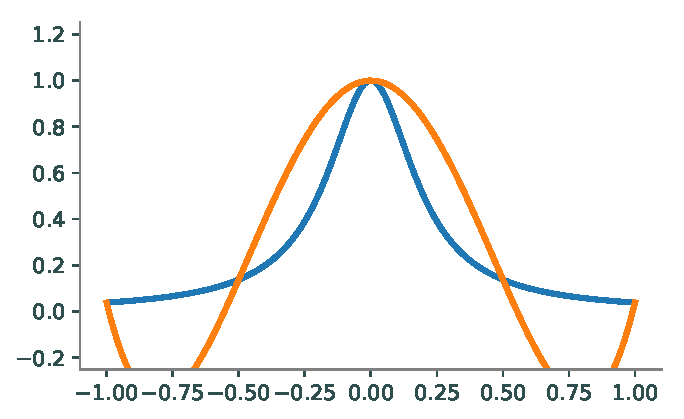
\includegraphics[width=\linewidth]{figures/bad_interp1.pdf}
    \caption{Interpolation using 5 equally spaced points.}
    \label{fig:bad1}
\end{subfigure}%
\begin{subfigure}{.5\textwidth}
    \centering
    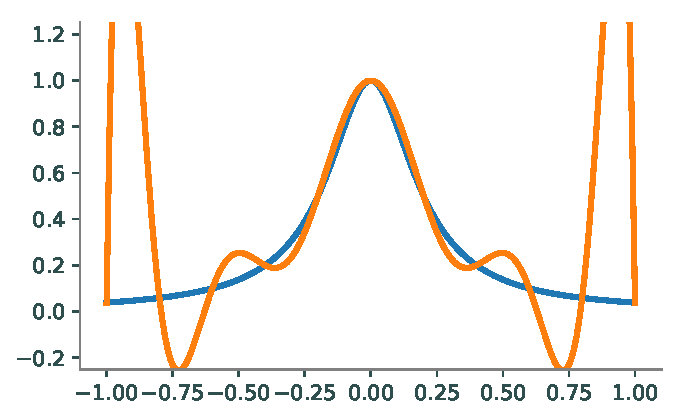
\includegraphics[width=\linewidth]{figures/bad_interp2.pdf}
    \caption{Interpolation using 11 equally spaced points.}
    \label{fig:bad2}
\end{subfigure}
\caption{Example of polynomial interpolation. Interpolation of Runge's function $f(x)=\frac{1}{1+25x^2}$ with differing numbers of equally spaced interpolating points.}
\label{fig:badinterp}
\end{figure}

\subsection*{Lagrange interpolation} %------------------------------------------------------------------------------------------------------------------------------------------------
Given a set $\{x_i\}_{i=1}^n$ of $n$ points to interpolate, a family of $n$ basis functions with the following property, is constructed:
\[
L_j(x_i) = \begin{cases} 0 &\mbox{ if } i \neq j\\ 1 &\mbox{ if } i =j \\ \end{cases}.
\]

Once each of the $n$ polynomials in this family of basis functions is known, they can be combined with the y-values $y_i=f(x_i)$ of the function to be interpolated in the following manner:
\begin{equation}
\label{equa:poly}
p(x) = \sum_{j=1}^n y_j L_j(x)
\end{equation}
This will create the unique interpolating polynomial.

The Lagrange form of this family of basis functions is
\begin{equation}
\label{equa:lagrange}
L_j(x) = \frac{\displaystyle\prod_{k=1, k \neq j}^n (x-x_k)}{\displaystyle\prod_{k=1, k \neq j}^n (x_j-x_k)}
\end{equation}
Each of these Lagrange basis functions is of degree $n-1$ and has the necessary properties as given above.
\emph{Lagrange interpolation} consists of computing the Lagrange basis functions then combining them with the y-values.

Since polynomials are typically represented in their expanded form with coefficients on each of the terms, it may seem like the best option when working with polynomials would be to use Sympy, or Numpy's
\li{poly1d} class to compute the coefficients of the interpolating polynomial individually.
This is rarely the best approach, however, since expanding out the large polynomials that are required can quickly lead to instability (especially when using large 
numbers of interpolating points).
Instead, it is usually best just to leave the polynomials in unexpanded form (which is still a polynomial, just not a pretty-looking one), and compute values of the polynomial directly from this unexpanded form. 

\begin{lstlisting}
# Evaluate the polynomial (x-2)(x+1) at 10 points without expanding the expression.
>>> pts = np.arange(10)
>>> (pts - 2) * (pts + 1)
array([ 2,  0,  0,  2,  6, 12, 20, 30, 42, 56])
\end{lstlisting}
In the given example, there would have been no instability if the expression had actually been expanded but in the case of a large polynomial, stability issues can dominate the computation.
Although the coefficients of the interpolating polynomials will not be explicitly computed in this lab, polynomials are still being used, albeit in a different form.

\begin{problem}
Write a function that uses the Lagrange method to find an interpolating polynomial for a set of data points and evaluates the calculated polynomial at specified values.
This function should accept two Numpy arrays which contain the $x$ and $y$ values of the interpolation points as well as a Numpy array of values (of length $m$) at which the interpolating polynomial 
will be evaluated.
Your function should return a Numpy array of the evaluated points.
The following steps will help in writing your function:
\begin{enumerate}
\item Compute the denominator of each $L_j$ (as in Equation \ref{equa:lagrange}) .
\item Using the previous step, evaluate each $L_j$ at all points in the compuational domain (this will give you $m$ values for each of the $n$ $L_j$ functions).
\item Combine all of these values as in Equation \ref{equa:poly}, this will give you the final array of length $m$.
\end{enumerate}
Note that steps one and two can be done in the same loop.
You may find the function \li{np.delete()} to be useful while writing this method.

You can test your function by plotting Runge's function $f(x)=\frac{1}{1+25x^2}$ and your interpolating polynomial on the same plot for different values of $n$ equally spaced interpolating values then comparing 
your plot to the plots given in Figure \ref{fig:badinterp}.
\label{prob:lagrange}
\end{problem}

The Lagrange form of polynomial interpolation is useful in some theoretical contexts and is easier to understand than other methods, however, it has some serious drawbacks that prevent it from being a 
useful method of interpolation.
First, Lagrange interpolation is $O(n^2)$ where other interpolation methods are $O(n^2)$ (or faster) at startup but only $O(n)$ at run-time, 
Second, Lagrange interpolation is an unstable algorithm which causes it to return innacurate answers when larger numbers of interpolating points are used.
Thus, while useful in some situations, Lagrange interpolation is not desirable in most instances.

\subsection*{Barycentric Lagrange interpolation}
Barycentric Lagrange interpolation is simple variant of Lagrange interpolation that performs much better than plain Lagrange interpolation.  
It is essentially just a rearrangement of the order of operations in Lagrange multiplication which results in vastly improved perfomance, both in speed and stability.

Barycentric Lagrange interpolation relies on the observation that each basis function $L_j$ can be rewritten as
\[
L_j(x) = \frac{w(x)}{(x-x_j)}w_j
\]
where 
\[
w(x) = \prod_{j=1}^n (x-x_j)
\]
and
\[
w_j = \frac{1}{\prod_{k=1, k \neq j}^n (x_j-x_k)}.
\]
The $w_j$'s are known as the \emph{barycentric weights}.

Using the previous equations, the interpolating polynomial can be rewritten
\[
p(x) = w(x) \sum_{j=1}^n \frac{w_j y_j}{x-x_j}
\]
which is the \emph{first barycentric form}.
The computation of $w(x)$ can be avoided by first noting that
\[
1 = w(x) \sum_{j=1}^n \frac{w_j}{x-x_j}
\]
which allows the interpolating polynomial to be rewriten as
\[
p(x) = \frac{\displaystyle\sum_{j=1}^n \frac{w_j y_j}{x-x_j}}{\displaystyle\sum_{j=1}^n \frac{w_j}{x-x_j}}
\]
This form of the Lagrange interpolant is known as the \emph{second barycentric form} which is the form used in Barycentric Lagrange interpolation.
So far, the changes made to Lagrange interpolation have resulted in an algorithm that is $O(n)$ once the barycentric weights ($w_j$) are known.
The following adjustments will improve the algorithm so that it is numerically stable and later discussions will allow for the quick addition of new interpolating points after startup.

The second barycentric form makes it clear that any factors that are common to the $w_k$ can be ignored (since they will show up in both the numerator and denominator).
This allows for an important improvement to the formula that will prevent overflow error in the arithmetic.
When computing the barycentric weights, each element of the product $\prod_{k=1, k \neq j}^n (x_j-x_k)$ should be multiplied by $C^{-1}$, where $4C$ is the width of the interval being interpolated 
(C is known as the \emph{capacity} of the interval).
In effect, this scales each barycentric weight by $C^{1-n}$ which helps to prevent overflow during computation.
Thus, the new barycentric weights are given by
\[
w_j = \frac{1}{\prod_{k=1, k \neq j}^n \left[(x_j-x_k)C\right]}.
\]
Once again, this change is possible since the extra factor $C^{1-n}$ is cancelled out in the final product.
This process is summed up in the following code:

\begin{lstlisting}
# Given a Numpy array xint of interpolating x-values, calculate the weights.
>>> n = len(xint)                   # Number of interpolating points.
>>> w = np.ones(n)                  # Array for storing barycentric weights.
# Calculate the capacity of the interval.
>>> C = (np.max(xint) - np.min(xint)) / 4
    
>>> shuffle = np.random.permutation(n-1)
>>> for j in range(n):
>>>     temp = (xint[j] - np.delete(xint, j)) / C
>>>     temp = temp[shuffle]        # Randomize order of product.
>>>     w[j] /= np.product(temp)
\end{lstlisting}

The order of \li{temp} was randomized so that the arithmetic does not overflow due to poor ordering (if standard ordering is used, overflow errors can be encountered since all 
of the points of similar magnitude are multiplied together at once).
When these two fixes are combined, the Barycentric Algorithm becomes numerically stable.

\begin{problem}
\label{prob:barycentric}
Create a class that performs Barycentric Lagrange interpolation.
The constructor of your class should accept two Numpy arrays which contain the $x$ and $y$ values of the interpolation points.
Store these arrays as class attributes.
The constructor should compute the corresponding barycentric weights and store the resulting array as a class attribute.
When storing the arrays as class attributes be sure that the relative ordering of the arrays remains unchanged.

Write the \li{__call__} method of your class so that it accepts a Numpy array of values at which to evaluate the interpolating polynomial and returns an array of the evaluated points.
Your class can be tested in the same way as the Lagrange function written in Problem \ref{prob:lagrange}
\end{problem}

\begin{warn}
As currently explained and implemented, the Barycentric class from Problem \ref{prob:barycentric} will fail when a point to be evaluated exactly matches one of the x-values of the interpolating points.
This happens because a divide by zero error is encountered in the final step of the algorithm.
The fix for this, although not required here, is quite easy.
To repair this error, just keep track of any problem points and replace the final computed value with the corresponding y-value (since this is a point that is exactly interpolated).
If you do not implement this fix, just be sure not to pass in any points that exactly match your interpolating values.
\end{warn}

Another advantage of the barycentric method is that it allows for the addition of new interpolating points in $O(n)$ time.
Given a set of existing barycentric weights $\{ w_j\}_{j=1}^n$ and a new interpolating point $x_i$, the new barycentric weight is given by
\[
w_i = \frac{1}{\prod_{k=1}^n (x_i-x_k)}.
\]
In addition to calculating the new barycentric weight, all existing weights should be updated as follows $w_j=\frac{w_j}{x_j-x_i}$.

\begin{problem}
\label{prob:add weights}
Include a method in the class written in Problem \ref{prob:barycentric} that allows for the addition of new interpolating points by updating the barycentric weights.
Your function should accept two Numpy arrays which contain the $x$ and $y$ values of the new interpolation points.
Update and store the old weights then extend the class attribute arrays that store the weights, and the $x$ and $y$ values of the interpolation points with the new data.
When updating all class attributes, make sure to maintain the same relative order.
\end{problem}

The implementation outlined here calls for the y-values of the interpolating points to be known during startup, however, these values are not needed until run-time
This allows the y-values to be changed without having to recompute the barycentric weights.
This is an additional advantage of Barycentric Lagrange interpolation.

\subsection*{Scipy's Barycentric Lagrange class}
Scipy includes a Barycentric interpolator class.
This class includes the same functionality as the class described in Problems \ref{prob:barycentric} and \ref{prob:add weights} in addition to the ability to update the y-values of the interpolation points.
The following code will produce a figure similar to Figure \ref{fig:bad2}.
\begin{lstlisting}
>>> from scipy.interpolate import BarycentricInterpolator

>>> f = lambda x: 1/(1+25 * x**2)   # Function to be interpolated.
# Obtain the Chebyshev extremal points on [-1,1].
>>> n = 11
>>> pts = np.linspace(-1, 1, n)
>>> domain = np.linspace(-1, 1, 200)

>>> poly = BarycentricInterpolator(pts[:-1])
>>> poly.add_xi(pts[-1])          # Oops, forgot one of the points.
>>> poly.set_yi(f(pts))           # Set the y values.

>>> plt.plot(domain, f(domain))
>>> plt.plot(domain, poly.eval(domain))
\end{lstlisting}

\begin{comment} # Potential timing problem comparing student written barycentr, lagrange and Scipy's Lagrange.  Superceded by later problem which also includes Chebyshev.
\begin{problem}
Compare the runtime and error of your Lagrange and Barycentric methods with Scipy's Barycentric class by writing two functions, one comparing error and the other run-time.
Both functions should accept a callable function to interpolate and an integer designating how many interpolating points should be used.
All computations should be made on 200 equally spaced points on the interval $[-1, 1]$ with the interpolating points coming from the Chebyshev roots.
Both functions should print the runtime or error of the interpolation for all three methods with an accompanying description (so that it is obvious which time/error corresponds to which method).
When calculating error, use \li{np.linalg.norm()} with \li{ord=np.inf}.
\end{problem}
\end{comment}

\begin{figure}[H]
\captionsetup[subfigure]{justification=centering}
\captionsetup{justification=centering}
\centering
\begin{subfigure}{.5\textwidth}
    \centering
    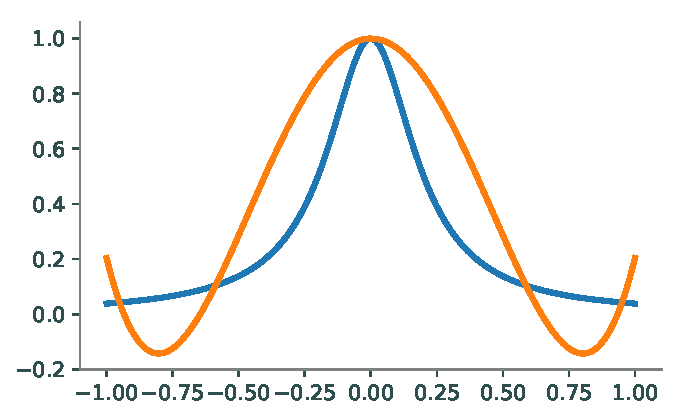
\includegraphics[width=\linewidth]{figures/good_interp1.pdf}
    \caption{Polynomial using 5 Chebyshev roots.}
    \label{fig:good1}
\end{subfigure}%
\begin{subfigure}{.5\textwidth}
    \centering
    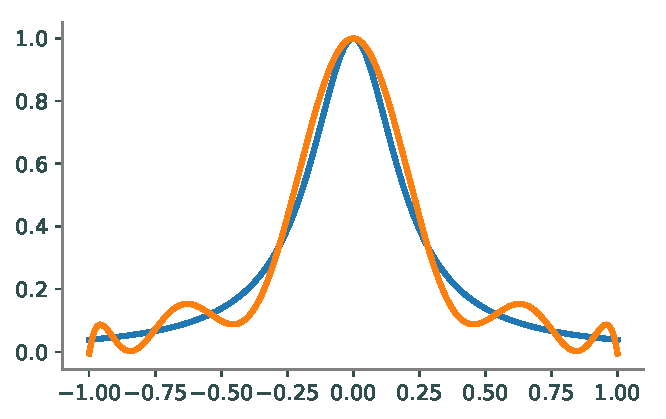
\includegraphics[width=\linewidth]{figures/good_interp2.pdf}
    \caption{Polynomial using 11 Chebyshev roots.}
    \label{fig:good2}
\end{subfigure}
\caption{Example of overcoming Runge's phenomenon by using Chebyshev nodes for interpolating values.
Plots made using Runge's function $f(x)=\frac{1}{1+25x^2}$.
Compare with Figure \ref{fig:badinterp}}
\label{fig:goodinterp}
\end{figure}

\section*{Chebyshev Interpolation}
\subsection*{Chebyshev Nodes}
As has been mentioned previously, the Barycentric version of Lagrange interpolation is a stable process that does not accumulate large errors, even with extreme inputs.
However, polynomial interpolation itself is, in general, an ill-conditioned problem.
Thus, even small changes in the interpolating values can give drastically different interpolating polynomials.
In fact, poorly chosen interpolating points can result in a very bad approximation of a function.
As more points are added, this approximation can worsen.
This increase in error is called \emph{Runge's phenomenon}.

The set of equally spaced points is an example of a set of points that may seem like a reasonable choice for interpolation but in reality produce very poor results.
Figure \ref{fig:badinterp} gives an example of this using Runge's function.
As the number of interpolating points increases, the quality of the approximation deteriorates, especially near the endpoints.

Although polynomial interpolation has a great deal of potential error, a good set of interpolating points can result in fast convergence to the original function as the number of interpolating points is increased.
One such set of points is the Chebyshev extremal points which are related to the Chebyshev polynomials (to be discussed shortly).
%The $n$ Chebyshev roots on the interval $[a,b]$ are given by the formula $z_j=\frac{1}{2}(a+b + (b-a)\cos(\frac{\pi}{n}(j+\frac{1}{2})))$ for $j=0,1,\dots,n-1$.
The $n+1$ Chebyshev extremal points on the interval $[a,b]$ are given by the formula $y_j=\frac{1}{2}(a+b + (b-a)\cos(\frac{j\pi}{n}))$ for $j=0,1,\dots,n$.
These points are shown in Figure \ref{fig:extrema}.
One important feature of these points is that they are clustered near the endpoints of the interval, this is key to preventing Runge's phenomenon.

\begin{problem}
Compare the error of interpolation using equally spaced points and interpolation using the Chebyshev extrema by writing a function that does the following:
\begin{itemize}
\item Interpolates Runge's function six times on the interval $[-1,1]$, three times using equally spaced points and three using the Chebyshev extrema.
\item Performs the interpolations with $n=[10,50,100]$ (note that for the Chebyshev extrema, the given definition uses $n+1$ interpolating values).
\item Plots each of the interpolating polynomial (for a total of six plots).
\item Prints the error of the interpolation on a domain using 500 equally spaced points.  When printing the error, it should be clear which error belongs to which value of $n$ and to which method.
\end{itemize}
Use Scipy's BarycentricLagrange class to perform all of the interpolation.
When calculating the error, use \li{scipy.linalg.norm()} with \li{ord=np.inf}.
\end{problem}

\begin{figure}
\centering
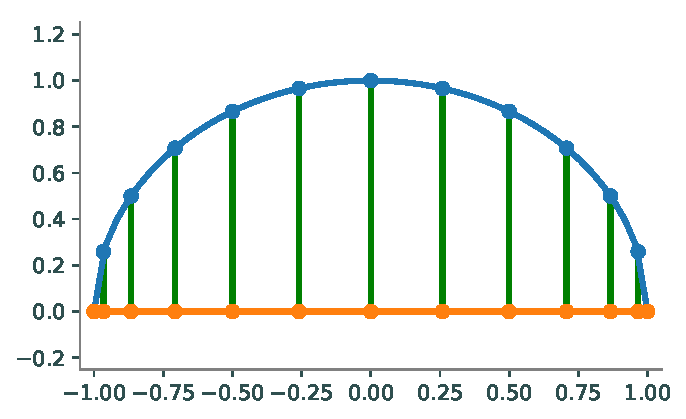
\includegraphics{figures/extrema.pdf}
\caption{The Chebyshev extremal points.  The $n$ points where the Chebyshev polynomial of degree $n$ reaches its local extrema.
These points are also the projection onto the x-axis of $n$ equally spaced points around the unit circle.}
\label{fig:extrema}
\end{figure}

\subsection*{Chebyshev Polynomials}
The Chebyshev roots and Chebyshev extremal points are closely related to a set of polynomials known as the Chebyshev polynomials.
The first two Chebyshev polynomials are defined as $T_0(x)=1$ and $T_1(x)=x$.
The remaining polynomials are defined by the recursive algorithm $T_{n+1}(x)=2xT_n(x)-T_{n-1}(x)$.
The Chebyshev polynomials form a complete basis for the polynomials in $\mathbb{R}$ which means that for any polynomial $p(x)$,  there exists a set of unique coefficients $\{a_k\}_{k=0}^n$
such that
\[
p(x) = \sum_{k=0}^n a_kT_k.
\]

Finding the Chebyshev representation of an interpolating polynomial is a slow process (dominated by matrix multiplication or solving a linear system), but when the interpolating values are the 
Chebyshev extrema, there exists a fast algorithm for computing the Chebyshev coefficients of the interpolating polynomial.
This algorithm is based on the Fast Fourier transform which has temporal complexity $O(n\log n)$.
Given the $n+1$ Chebyshev extremal points $y_j=\cos(\frac{j\pi}{n})$ for $j=0,1,\dots,n$ and a function $f$, the unique n-degree interpolating polynomial $p(x)$ is given by
\[
p(x)=\sum_{k=0}^na_kT_k
\]
where 
\[
a_k = \gamma_k \Re \left[ DFT(f(y_0), f(y_1),\dots, f(y_{2n-1}))\right]_k.
\]
Note that although this formulation includes $y_j$ for $j>n$, there are really only $n+1$ distinct values being used since $y_{n-k}=y_{n+k}$.
Also, $\Re$ denotes the real part of the Fourier transform and $\gamma_k$ is defined as
\[
\gamma_k = 
\begin{cases}
1 & k\in \{0,n\} \\
2 & \text{otherwise.}
\end{cases}
\]

\begin{problem}
Write a funtion that finds the Chebyshev coefficients for the degree $n$ interpolating polynomial of a function \li{f}.
Your function should accept a callable function \li{f} and an integer $n$ which denotes the degree of the interpolating polynomial.
Make the function return a Numpy array of the Chebyshev coefficients.
The functions \li{np.real()} and \li{np.fft.fft()} will be helpful in writing your function.
When using Numpy's \li{fft()} function, you will need to divide every entry of the resulting array by the scaling factor $\frac{1}{2n}$ since it is missing from Numpy's implementation.
\end{problem}

Once the coefficients of the Chebyshev polynomial have been computed, there exists a fast algorithm (discussed in Additional Materials) for evaluating the polynomials.
Numpy's \li{chebyshev} module contains a method for doing this.
\begin{lstlisting}
from numpy.polynomial.chebyshev import chebval

>>> domain = np.linspace(-1, 1, 5)
>>> f = lambda x: x**4              # Function to interpolate.
>>> coeffs = chebyshv_coeffs(f, 4)  # Function from Problem 6.
>>> print(coeffs)
[  3.75000000e-01  -5.88784672e-17   5.00000000e-01   5.88784672e-17
   1.25000000e-01]

>>> chebval(domain, coeffs)         # Evaluate at the points in domain.
[ 1.      0.0625  0.      0.0625  1.    ]
\end{lstlisting}

Although not covered here, Numpy's \li{chebyshev} module has a lot of useful functions for working with Chebyshev polynomials.
Some of the methods include fast implementations of polynomial operations such as addition and division plus methods for integration and multiplication.

\section*{Lagrange vs. Chebyshev}
As was previously stated, Barycentric Lagrange interpolation is $O(n^2)$ at startup and $O(n)$ at runtime while Chebyshev interpolation is $O(n\log n)$, this improved speed is one of the greatest
advantages of Chebyshev interpolation.
Chebyshev interpolation is also more accurate than Barycentric interpolation, even when using the same points.
Despite these significant advantages in accuracy and temporal complexity, Barycentric Lagrange interpolation has one very important advantage over Chebyshev interpolation.
Barycentric interpolation can be used on any set of interpolating points while Chebyshev is restricted to the Chebyshev nodes.
In general, because of their better accuracy, the Chebyshev nodes are more desirable for interpolation, but there are situations when the Chebyshev nodes are not available or when specific 
points are needed in an interpolation.
In these cases, Chebyshev interpolation is not possible and Barycentric Lagrange interpolation must be used.

\begin{problem}
Investigate the claims made in the previous section by writing two different functions, one to compare error and the other to compare time.
This function should accomplish this by doing the following:
\begin{itemize}
\item Interpolate Runge's function on the interval $[-1,1]$ using your Lagrange function, your Barycentric Lagrange class, Scipy's Barycentric class and Chebyshev interpolation.
\item Use the Chebyshev extremal points for the interpolating values.
\item Print the error or time required to run the function for each of the methods for $n=[500,1000,1500]$ interpolating values.
Be sure to clearly label the method and value of $n$ being used for each value printed.
\item Always evaluate at 200 equally spaced points in the domain.
\end{itemize}
Use \li{scipy.linalg.norm()} with \li{ord=np.inf} and the Chebyshev extremal points.
Note that if \li{inf} appears in any of your compuatations \li{scipy.linalg.norm()} will raise an error, in this case print the error as \li{inf} (you may need to use a \li{try} \li{except} block for some of the methods).
\end{problem}


\section*{Utah Air Quality}
The Utah Department of Environmental Quality has air quality stations throughout the state of Utah that measure the concentration of particles found in the air.
One particulate of particular interest is $PM_{2.5}$ which is a set of extremely fine particles known to cause tissue damage to the lungs.
The file \texttt{airdata.npy} has the hourly concentration of $PM_{2.5}$ in micrograms per cubic meter for a particular measuring station in Salt Lake County for the year 2016.
The given data presents a fairly smooth function which can be reasonably approximated by an interpolating polynomial.
Although Chebyshev interpolation would be preferable (because of its superior speed and accuracy), it is not possible in this case because the data is not continous and the information at the Chebyshev nodes
is not known.
In order to get the best possible interpolation, it is still preferable to use points close to the Chebyshev extrema with Barycentric interpolation.
The following code will take the $n+1$ Chebyshev extrema and find the closest match in the non-continuous data found in the variable \li{data} then calculate the barycentric weights.

\begin{lstlisting}
>>> fx = lambda a, b, n: .5*(a+b + (b-a) * np.cos(np.arange(n+1) * np.pi / n))
>>> a, b = 0, 366 - 1/24
>>> domain = np.linspace(0, b, 8784)
>>> points = fx(a, b, n)
>>> temp = np.abs(points - domain.reshape(8784, 1))
>>> temp2 = np.argmin(temp, axis=0)

>>> poly = barycentric(domain[temp2], data[temp2])
\end{lstlisting}

\begin{problem}
Write a function that interpolates the given data along the whole interval at the closest approximations to the $n+1$ Chebyshev extremal nodes.
The function should accept $n$, perform the Barycentric interpolation then plot the original data and the approximating polynomial on the same domain on two seperate subplots.
Your interpolating polynomial should give a fairly good approximation starting at around 50 points.
Note that beyond about 200 points, the given code will break down since it will attempt to return multiple of the same points causing a divide by 0 error.
If you did not perform the fix suggested in the Warning box, make sure not to pass in any points that exactly match the interpolating values.
\end{problem}
\pagebreak


\section*{Additional Materials}
The Clenshaw Algorithm is a fast algorithm commonly used to evaluate a polynomial given its representation in Chebyshev coefficients.
This algorithm is based on the recursive relation between Chebyshev polynomials and is the algorithm used by Numpy's \li{chebyshev} package.

\begin{algorithm}
\begin{algorithmic}[1]
\Procedure{ClenshawRecursion}{$x, a$}
	\State $u_{n+1} \gets 0$
	\State $u_{n} \gets 0$
	\State $k \gets n-1$
	\While{$k \geq 1$}
		\State $u_k \gets 2 x u_{k+1} - u_{k+2} + a_k$
		\State $k \gets k-1$
	\EndWhile
	\State \pseudoli{return} $a_0 + x u_1 -u_2$
\EndProcedure
\end{algorithmic}
\caption{Accepts an array $x$ of points at which to evaluate the polynomial and an array $a=[a_0,a_1,\dots,a_{n-1}]$ of Chebyshev coefficients.}
\label{alg:clenshaw_recursion}
\end{algorithm}


%%%%%%%%%%%%%%%%%%%%%%%%%%%%%%%%%%%%%%%%%%%%%%%%%%%%%%%%%%%%%%%%%%%%%%%%%%%%%%%%%
% The following is some unincluded material from the old Chebyshev Polynomial lab that expands on the material contained in the current lab, some of it may be useful for future iterations of this lab.

\begin{comment} %This section gives a more complete introduction to Chebyshev polynomials including their orthogonality.
This sort of interpolation is also related to what are called the Chebyshev polynomials.
Chebyshev Polynomials can be used very nicely to approximate functions on $[ -1, 1 ]$ and, with proper scaling, can be used to approximate reasonably well-behaved functions on any interval.
The $k$'th Chebyshev polynomial is commonly written $T_k \left( x \right)$.
One way to define the Chebyshev Polynomials is that the $k$'th Chebyshev polynomial on the unit circle is the real part of the function $z^k$ on the unit circle.
More precisely, let $z(x) = t + i \sqrt{1 - x^2}$, then the $k$'th Chebyshev polynomial on $[-1, 1]$ is the real part of the polynomial $x^k$.
We can write this real part explicitly as
\[T_k \left( x \right) = \frac{1}{2} \left( z^k + z^{-k} \right) = \cos \left( k \cos^{-1} \left( x \right) \right)\]
Notice that, as this function has been defined, the Chebyshev polynomial of order $k$ on an interval takes values of $1$ and $-1$ at the $k+1$ chebyshev points corresponding to interpolation with a polynomial of order $k$ on that interval.
The first few Chebyshev polynomials are shown in Figure \ref{fig:cheb_polys}.

These polynomials are orthogonal with respect to the integral inner product
\[\langle f, g \rangle = \int_{-1}^1 \frac{1}{\sqrt{1 - x^2}} f\left( x \right) g\left( x \right) dx\]
This inner product allows us to write many functions as an infinite series of Chebyshev polynomials.
In particular, we can write any polynomial as a finite series of Chebyshev polynomials.
As it turns out, it is relatively easy to compute the Chebyshev series representation of an interpolating polynomial for a function on a given interval.
These approximations converge to the function we are approximating nearly as well as the partial sums of the infinite series formed using the inner product above, so, in practice, we will use them instead.

It can be shown that the Chebyshev polynomials follow the following recurrence relation: $ T_{k+1} \left( x \right) = 2 x T_k \left( x \right) - T_{k-1}$.
$T_0 \left( x \right)$ is equal $1$ and $T_1 \left( x \right)$ is equal to $x$ (still working on the interval $[-1, 1]$.)
\end{comment}

\begin{comment} %This section includes a more mathematical introduction to the connection between Fourier series and Chebyshev Polynomials.
\section*{Chebyshev Polynomials and Fourier Series}
In looking at the plots of the Chebyshev polynomials you may have noticed that the Chebyshev polynomials take alternating values of $1$ and $-1$ at the Chebyshev points on the interval $[-1,1]$ similar to how the functions $\cos\left(k x \right)$ change between $-1$ and $1$ on equispaced points in the interval $[ 0 , \pi ]$.
Recall that, as mentioned above, $T_k \left( x \right) = \cos \left( k \cos^{-1} \left( x \right) \right)$.
For discrete samples, this means that the Chebyshev coefficients for the interpolating polynomial through a function at the Chebyshev nodes has the same coefficients as the discrete cosine series would at the points $\cos^{-1} x$ where $x$ is a chebyshev node.
In practice this means we can compute an array of samples of a function at the Chebyshev nodes of the interval $[-1, 1]$, then compute the discrete cosine transform to get the corresponding coefficients to the Chebyshev interpolation.
This is very helpful since the discrete cosine transform is a close relative of the discrete Fourier transform.
\li{scipy.fftpack} and \li{pyfftw} both include discrete cosine transforms as \li{scipy.fftpack.dct} and \li{pyfftw.interfaces.scipy_fftpack.dct} respectively.
The discrete cosine transform is defined a little differently than the coefficients we need here.
There are several different versions of the discrete cosine transform.
Using the inverse discrete cosine transform of type 1 on an array $y$ of length $N$ will give us an array $x$ of values such that
\[y_k = z_0 + 2 \sum_{n=1}^{N-2} z_n \cos\left(\frac{\pi k n}{N-1}\right) + \left(-1\right)^k z_{N-1}\]
where $z = \frac{x}{2 \left(N - 1\right)}$.
To obtain the Chebyshev coefficients, we desire to find the vector $a$ of coefficients $a_n$ such that
\[y_k = \sum_{n=0}^{N-1} a_n \cos\left(\frac{\pi k n}{N-1}\right)\]
This means that, given the vector $x$, we can obtain $a$ by dividing all the terms of $x$ by $N-1$, and then dividing the first and last entries of $x$ by 2.
This means that we can obtain the coefficients of the Chebyshev interpolant using the following steps:

\begin{itemize}

\item Sample the function you desire to approximate at the Chebyshev nodes.
Make sure you use the sampled values in the order that corresponds to the chebyshev nodes when sorted in \emph{descending} order and not ascending order.

\item Compute the inverse discrete cosine transform of the data.
Use the option \li{type=1} to tell either scipy or pyfftw the version of the discrete cosine transform you want to use.

\item Divide all the coefficients by $\left( N - 1 \right)$ where $N$ is the number of nodes used.

\item Divide the first and last coefficient by $2$.

\end{itemize}

\begin{warn}
Often it is customary in computation to use values in ascending order.
When you compute the Chebyshev coefficients for the interpolatng polynomial through a set of points you will need the samples from the points sorted in descending order, not ascending order.
\end{warn}
\end{comment}

\begin{comment} %Potential problem and discussion exploring convergence of polynomial interpolation.
\begin{problem}
\label{prob:cheb_interpolations}
We will briefly consider the rate of convergence of these polynomial approximations.
Compute the coefficients for the interpolating Chebyshev series for the function $\cos x$ on the interval $[-1, 1]$.
This approximation converges very rapidly, so the first $20$ terms or so should be more than enough.
How many of these coefficients have absolute value greater than $10^{-14}$?
How close does your series approximate the actual function?

Now compute the coefficients for a degree $100000$ polynomial approximating the function
\[\sin \left( \frac{1}{x} \right) \sin \left( \frac{1}{\sin \left( \frac{1}{x} \right)} \right) \]
on the interval $[-1, 1]$.
How large are the last $10$ coefficients in the series?
Use NumPy's Chebyshev class to plot this function at $100001$ equispaced points on the interval $[-1, 1]$.
Plot it with the original function.
Compare the two.
How close are they?
Notice how the interpolating polynomial is able to approximate the original function about as well as the discrete sample of the original function.
\end{problem}

Problem \ref{prob:cheb_interpolations} also illustrates an interesting principle.
These series converge more quickly when a function is infinitely differentiable everywhere in the complex plane (the proper term for a function like this is "entire").
For functions that do not satisfy this property, it can be shown (roughly speaking) that the rate of convergence depends on how many times differentiable the function is on the interval of interpolation.
For a less well-behaved function like the one considered in the second half of Problem \ref{prob:cheb_interpolations} the coefficients converge much more slowly.
The last $10$ coefficients for the interpolant of degree $2^{23} - 1$ are still
\begin{lstlisting}
[9.52973125e-08,  -1.89451973e-09,  -7.42182166e-08,
 1.89319137e-09,   5.26564839e-08,  -1.89451836e-09,
 -3.13050802e-08,   1.89319005e-09,   1.03700608e-08,
 -9.47258778e-10]
\end{lstlisting}
\end{comment}
